\chapter{Introduksjon}
%--------------------MÅ INN I HOVEDRAPPORT------------------------------------------
Rotårsaksanalyser er et lite brukt verktøy innen informasjonssikkerhet, men er av økende betydning. Vanlig tilnærming til informasjonssikkerhetsstyring er å utføre en risiko- og sårbarhetsanalyse (ROS-analyse) for så å gjennomføre tiltak som fører risikoene til et akseptabelt nivå. En annen hyppig brukt tilnærming er hendelseshåndtering der en planlegger hvordan det skal responderes på hendelser etter de er inntruffet. Rotårsaksanalyse skiller seg fra disse ved å gå i dybden på problemet, kartlegge hva slags rotårsaker som står bak, og innføre tiltak for å fjerne disse helt.
%%%%%%%%%%%%%%%%%%%%%%%%%%%%%%%%%%%%%%%%%%%%%%%%%%%%%%%%%%%%%%%%%%%%%%%%%%%%%%%%%%%%%

\section{Oppgavebeskrivelse}
Denne rapporten er en delrapport i en større oppgave om rotårsaksanalyse. Dette caset går inn på rotårsaken til misbruk av NTNU sine ressurser og infrastruktur til å grave kryptovaluta. De to siste årene har både verdien og antallet av kryptovaluta økt drastisk. Det finnes per dags dato over 1500 forskjellige kryptovalutaer. Kryptovaluta blir "minet", eller gravet ut, ved bruk av regnekraft. Dette betyr at enhver datamaskin kan delta i utgravingen. Etterhvert vil vanskelighetsgraden for å grave ut nye "coins", eller mynter, øke. Når vanskelighetsgraden øker trenger en mer datakraft og større maskinrigger til å grave ut mynter. 

NTNU forvalter stor regnekraft spredt på flere lokasjoner. NTNU har også hatt supermaskiner før, de har en nå og de får nå en ny supermaskin. Supermaskiner er store datamaskiner på størrelse med et rom, og har enorm datakraft. Disse er spesielt attraktive for aktører å misbruke til å grave etter mynter. Siden trenden har økt de siste årene, og NTNU er i besittelse av mye regnekraft, må NTNU aktivt jobbe for å beskytte infrastrukturen. 

Siden dette er av økende trend, og Seksjon for Digital Sikkerhet har oppdaget at noe av infrastrukturen har blitt brukt til utgraving av kryptovaluta, vil de undersøke måter å eliminere dette misbruket. 

Denne analysen går ut på å identifisere rotårsaken til den økende trenden å bruke NTNU sin infrastruktur til utgraving av kryptovaluta og foreslå tiltak for å eliminere den. I løpet av rapporten ønsker vi å svare på følgende forskningsspørsmål:

\begin{itemize}
    \item 
\end{itemize}

\section{Metode}
Metodebruken i denne analysen er delt inn i syv steg som vist i \hyperref[fig:prosess]{Figur 1} under. I hvert steg av denne prosessen brukes det ulike verktøy for å hjelpe til med å forstå problemet, finne rotårsak, og tilslutt implementere tiltak for å eliminere årsakene. 
\begin{figure}[H]
    \centering
    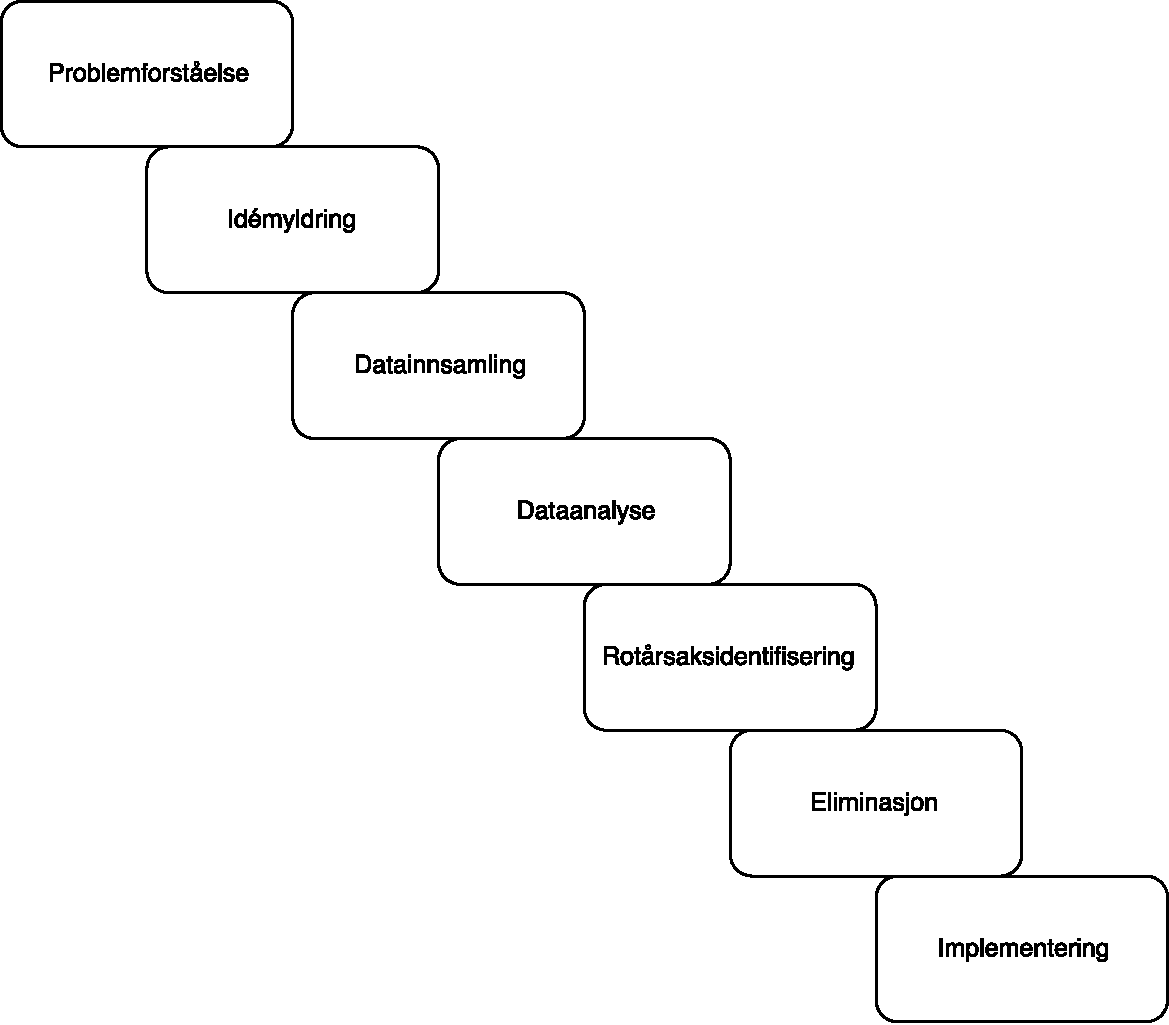
\includegraphics[scale=0.6]{case_1/bilder/prosess.pdf}
    \label{fig:prosess}
    \caption[Rotårsaksanalyseprosessen]{Rotårsaksanalyseprosessen definert av Andersen og Fagerli}
\end{figure}